\pdfbookmark{Общая характеристика работы}{characteristic}             % Закладка pdf
\section*{Общая характеристика работы}

\newcommand{\actuality}{\pdfbookmark[1]{Актуальность}{actuality}\underline{\textbf{\actualityTXT}}}
\newcommand{\progress}{\pdfbookmark[1]{Разработанность темы}{progress}\underline{\textbf{\progressTXT}}}
\newcommand{\aim}{\pdfbookmark[1]{Цели}{aim}\underline{{\textbf\aimTXT}}}
\newcommand{\tasks}{\pdfbookmark[1]{Задачи}{tasks}\underline{\textbf{\tasksTXT}}}
\newcommand{\aimtasks}{\pdfbookmark[1]{Цели и задачи}{aimtasks}\aimtasksTXT}
\newcommand{\novelty}{\pdfbookmark[1]{Научная новизна}{novelty}\underline{\textbf{\noveltyTXT}}}
\newcommand{\influence}{\pdfbookmark[1]{Практическая значимость}{influence}\underline{\textbf{\influenceTXT}}}
\newcommand{\methods}{\pdfbookmark[1]{Методология и методы исследования}{methods}\underline{\textbf{\methodsTXT}}}
\newcommand{\defpositions}{\pdfbookmark[1]{Положения, выносимые на защиту}{defpositions}\underline{\textbf{\defpositionsTXT}}}
\newcommand{\reliability}{\pdfbookmark[1]{Достоверность}{reliability}\underline{\textbf{\reliabilityTXT}}}
\newcommand{\probation}{\pdfbookmark[1]{Апробация}{probation}\underline{\textbf{\probationTXT}}}
\newcommand{\contribution}{\pdfbookmark[1]{Личный вклад}{contribution}\underline{\textbf{\contributionTXT}}}
\newcommand{\publications}{\pdfbookmark[1]{Публикации}{publications}\underline{\textbf{\publicationsTXT}}}


{\actuality} 

Инфракрасное излучение было открыто английским астрономом У.~Гершелем в 1800 году, и вскоре после этого были обнаружены такие его свойства, как способность поглощаться с выделением тепла и существование окон прозрачности атмосферы в некоторых спектральных диапазонах. Однако генерация когерентного излучения среднего ИК-диапазона (3--50 мкм) стала возможна только после изобретения лазеров и развития нелинейной оптики. В настоящее время для этих целей широко используются мощные одномодовые волоконные лазеры, которые благодаря сочетанию высокой пиковой (до 100~кВт) и средней (до 10~кВт) оптической мощности, высокому качеству пучка ($M^2 < 1.3$) и коэффициенту полезного действия (более 45\% от розетки) успешно конкурируют с твердотельными аналогами. Для преобразования их излучения в средний ИК--диапазон применяются нелинейно-оптические (н-о) кристаллы, позволяющие с помощью эффектов второго порядка (генерация разностной, суммарной частот) расширять доступный спектральный диапазон от ультрафиолета до среднего ИК. Особое место занимает область длин волн около $3$~мкм, поскольку в неё попадают пики поглощения воды, молекулярных связей, а также несколько окон прозрачности атмосферы. Поэтому излучение в данной спектральной области широко используется в медицине (дерматология, хирургия), спектроскопии, дистанционном зондировании атмосферы, лазерной связи в свободном пространстве~\cite{jean2003mid, haas2016advances, lambert2015differential, grillot2025progress}. Для генерации излучения в диапазоне 3 мкм используются различные твердотельные активные среды, включая кристалл Er:YAG, фторидное волокно Ho:ZBLAN, а также халькогениды (ZnS, ZnSe), легированные ионами Cr²⁺ или Fe²⁺.
%Такие лазеры активно применяется в коммерческих медицинских системах~\cite{bader2006indications, jean2003mid}.
Альтернативным методом, позволяющим создавать компактные и эргономичные устройства с волоконным инструментом, обеспечивающим возможность перестройки длины волны и узкую линию излучения, является генерация разностной частоты (ГРЧ) в кристалле ниобата лития с регулярной доменной структурой (PPLN) при накачке двумя импульсными волоконными лазерами, излучающими на длинах волн 1030~нм и 1560~нм, импульсы которых синхронизированы по времени и распространяются по одному оптическому волокну~\cite{larionov2021pp}.

Однако при создании стабильных и эффективных источников среднего ИК-диапазона следует учитывать две группы явлений, связанных с н-о и тепловыми процессами в оптических волокнах (ОВ) и н-о кристаллах.

Первая группа связана с синхронным распространением мощных оптических импульсов на двух длинах волн по ОВ, которое используется для доставки излучения к н-о кристаллу. С повышением пиковой мощности в ОВ проявляются н-о эффекты. Явления, обусловленные нелинейной поляризуемостью третьего порядка, такие как четырёхволновое смешение (ЧВС), приводят к искажению спектра и снижению мощности в исходных спектральных компонентах~\cite{agrawal2019}. В ОВ, не являющихся одномодовыми хотя бы на одной из длин волн излучения, картина ЧВС усложняется. В таких условиях возможно одновременное протекание как одномодового, так и межмодового ЧВС, поэтому необходимо выяснить, какие именно типы ЧВС реализуются в конкретной ситуации и почему они влияют друг на друга.


Помимо эффектов третьего порядка, в ОВ, несмотря на его центросимметричность, возможна реализация оптически индуцированных эффектов второго порядка, в частности, генерации второй гармоники (ГВГ)~\cite{osterberg1986dye}. Этот эффект снижает мощность излучения основной частоты, ухудшает качество пучка и уменьшает порог оптического разрушения нелинейно-оптических кристаллов. Механизм фотоиндуцированной ГВГ связан с формированием объёмной решётки квадратичной нелинейности при длительном облучении ОВ. Эффективность этого процесса определяется условиями фазового синхронизма, поэтому исследование эволюции соответствующих кривых фазового синхронизма (КФС) в процессе записи решётки может дать важную информацию о динамике её формирования и, в конечном итоге, о её микроскопической природе. Однако до настоящего времени такие экспериментальные исследования, особенно в отсутствие затравочного излучения второй гармоники (что типично для практических лазерных систем, где ГВГ является нежелательным эффектом), проведены не были.

Вторая группа явлений возникает при н-о преобразовании в н-о кристалле. Любой реальный кристалл обладает хоть и малым, но ненулевым коэффициентом оптического поглощения, причём на различных длинах волн излучения коэффициент также будет различаться. Например, для PPLN на длине волны 3 мкм коэффициент поглощения составляет порядка $10^{-2}~\text{см}^{-1}$, в то время как на длинах волн $1.03$~мкм и $1.56$~мкм он составляет $10^{-3}~\text{см}^{-1}$ и $10^{-4}~\text{см}^{-1}$ соответственно.~\cite{leidinger2015comparative} Оптическое поглощение лазерного излучения приводит к разогреву кристалла, изменению показателя преломления и нарушению условий фазового синхронизма, что снижает эффективность н-о преобразования. Для учёта и компенсации тепловых эффектов, таких, как индуцированная фазовая расстройка или термолинзирование, необходимо точное знание коэффициента поглощения. Перспективным методом его измерения является пьезоэлектрическая резонансная лазерная калориметрия (ПРЛК), позволяющая определять усреднённую температуру пьезоэлектрического кристалла по сдвигу частоты одной его собственных акустических мод, бесконтактно возбуждаемой внешним переменным электрическим полем за счёт обратного пьезоэлектрического эффекта~\cite{aloyan2022acoustic}. Для обработки температурных кинетик применяют три стандартных подхода: экспоненциальную методику, в которой коэффициент оптического поглощения определяют по кинетике нагрева; импульсную методику, основанную на анализе кинетики охлаждения; а также градиентную методику, основанную на сопоставлении скоростей изменения температуры при нагреве и остывании для одинакового разогрева. Общим недостатком этих подходов является то, что они не учитывают нестационарность температуры окружающей среды и коэффициента теплоотдачи, что приводит к существенному разбросу результатов.

Настоящая диссертационная работа посвящена исследованию н-о процессов при распространении мощных оптических импульсов по ОВ, а также тепловых процессов в н-о кристаллах, ограничивающих эффективность и стабильность гибридного источника излучения на длине волны 3~мкм.

\ifsynopsis
%Этот абзац появляется только в~автореферате.
%Для формирования блоков, которые будут обрабатываться только в~автореферате,
%заведена проверка условия \verb!\!\verb!ifsynopsis!.
%Значение условия задаётся в~основном файле документа (\verb!synopsis.tex! для
%автореферата).
\else
%Этот абзац появляется только в~диссертации.
%Через проверку условия \verb!\!\verb!ifsynopsis!, задаваемого в~основном файле
%документа (\verb!dissertation.tex! для диссертации), можно сделать новую
%команду, обеспечивающую появление цитаты в~диссертации, но~не~в~автореферате.
\fi

% {\progress}
% Этот раздел должен быть отдельным структурным элементом по
% ГОСТ, но он, как правило, включается в описание актуальности
% темы. Нужен он отдельным структурынм элемементом или нет ---
% смотрите другие диссертации вашего совета, скорее всего не нужен.

Таким образом, {\aim} диссертационной работы является исследование н-о эффектов второго и третьего порядка, развивающихся в ОВ доставки излучения, а также разработка подходов к повышению точности измерения коэффициента оптического поглощения в н-о кристаллах для источника излучения на длине волны вблизи 3~мкм.

Для~достижения поставленной цели необходимо было решить следующие {\tasks}:
\begin{enumerate}[beginpenalty=10000] % https://tex.stackexchange.com/a/476052/104425
  \item выяснить причины взаимного влияния процессов четырёхволнового смешения при распространении синхронизированных оптических импульсов двухволнового лазерного источника в маломодовом ОВ и разработать математическую модель, описывающую это взаимодействие;
  
  \item исследовать эволюцию кривых фазового синхронизма при фотоиндуцированной генерации второй гармоники в оптическом волокне в процессе формирования решётки нелинейной поляризуемости второго порядка и сопоставить экспериментальные результаты с модельными;

  \item проанализировать основные источники погрешности измерения коэффициента оптического поглощения в нелинейно-оптических кристаллах методом ПРЛК и предложить способы их компенсации.
\end{enumerate}


{\novelty}
\begin{enumerate}[beginpenalty=10000] % https://tex.stackexchange.com/a/476052/104425
  \item Установлено, что взаимное влияние одномодового и межмодового четырёхволнового смешения в маломодовом оптическом волокне обусловлено наличием у этих н-о процессов общей антистоксовой компоненты. Предложен метод подавления нежелательных спектральных компонент с помощью модового фильтра.
  
  \item Обнаружено, что в процессе формирования решётки квадратичной нелинейной восприимчивости при фотоиндуцированной генерации второй гармоники в германосиликатном ОВ ширина кривых фазового синхронизма монотонно уменьшается, их пик сдвигается к расстройке, определяемой фазовой самомодуляцией и кросс-модуляцией, при этом форма кривых синхронизма сохраняет выраженную асимметрию.  
  
  \item Для экспоненциального, импульсного и градиентного методов обработки температурных кинетик при разогреве н-о кристалла лазерным излучением предложены поправочные выражения, позволяющие компенсировать нестационарность температуры окружающей среды и коэффициента теплообмена.
  
\end{enumerate}

{\influence}:

\begin{enumerate}[beginpenalty=10000] 
	\item Предложенный метод подавления межмодового четырёхволнового смешения основан на использовании модового фильтра в виде участка одномодового ОВ, согласованного по модовому диаметру с ОВ доставки. Применение метода позволяет увеличить допустимую длину ОВ доставки с 2.5 м до 3.0 м без снижения эффективности генерации разностной частоты, что важно для создания практичных и функциональных лазерных источников среднего ИК-диапазона.
	
	\item Полученные зависимости эволюции кривых фазового синхронизма при оптическом полинге ОВ позволяют определить изменение фазовой расстройки в процессе формирования решётки квадратичной нелинейности. Это создаёт основу для будущих исследований по управлению фазой накачки с целью либо подавления паразитной ГВГ, либо её эффективной генерации.
	
	\item Разработанные поправочные выражения для обработки температурных кинетик н-о кристаллов при разогреве лазерным излучением позволяют снизить разброс измерений коэффициента оптического поглощения в три раза, повышая точность диагностики нелинейно-оптических кристаллов и достоверность оценки их теплового режима при работе в мощных лазерных системах.
	
\end{enumerate}
%
%{\methods} \ldots

{\defpositions}
\begin{enumerate}[beginpenalty=10000] % https://tex.stackexchange.com/a/476052/104425
  \item В маломодовом оптическом волокне взаимное влияние одномодового и межмодового четырёхволнового смешения синхронизированных оптических импульсов двухволнового лазерного источника обусловлено перекрытием спектров усиления их общих антистоксовых компонент.
  \item В процессе оптического полинга германосиликатного волокна излучением ближнего ИК-диапазона ширина кривых фазового синхронизма генерации второй гармоники монотонно уменьшается, а их пик сдвигается к расстройке, определяемой фазовой самомодуляцией и кросс-модуляцией. При этом выход эффективности ГВГ на постоянный уровень наступает до завершения эволюции кривых фазового синхронизма, поскольку указанные эффекты компенсируются одновременным ростом пиковой эффективности преобразования.
\end{enumerate}
%В папке Documents можно ознакомиться с решением совета из Томского~ГУ
%(в~файле \verb+Def_positions.pdf+), где обоснованно даются рекомендации
%по~формулировкам защищаемых положений.

{\reliability} полученных результатов обеспечивается высокой повторяемостью экспериментальных данных в пределах допустимой погрешности. Надёжность работы подтверждается применением современной приборной базы, а также сопровождением экспериментов численным моделированием. Основные результаты диссертации опубликованы в рецензируемых научных журналах.

\makeatletter
\setcounter{citeregistered}{0}
\makeatother

\ifnumequal{\value{bibliosel}}{0}
{%%% Встроенная реализация с загрузкой файла через движок bibtex8. (При желании, внутри можно использовать обычные ссылки, наподобие `\cite{vakbib1,vakbib2}`).
%    {\publications} 
    {\probation} Основные результаты по теме диссертации изложены
    в~XX~печатных изданиях,
    X из которых изданы в журналах, рекомендованных ВАК,
    X "--- в тезисах докладов.
    
    
    Общее число докладов на российских и международных конференциях~--- 16. Из них: 10 докладов на 8 международных конференциях (ICLO 2022, 2024; ALT 2025; LLPh 2023, 2025; Фотоника и информационная оптика 2022, 2023) и 6 докладов на 4 всероссийских конференциях (МФТИ 2022–2024; Самарская конкурс-конференция по оптике, лазерной физике и физике плазмы 2023).
}%
{%%% Реализация пакетом biblatex через движок biber
    \begin{refsection}[bl-author, bl-registered]
        % Это refsection=1.
        % Процитированные здесь работы:
        %  * подсчитываются, для автоматического составления фразы "Основные результаты ..."
        %  * попадают в авторскую библиографию, при usefootcite==0 и стиле `\insertbiblioauthor` или `\insertbiblioauthorgrouped`
        %  * нумеруются там в зависимости от порядка команд `\printbibliography` в этом разделе.
        %  * при использовании `\insertbiblioauthorgrouped`, порядок команд `\printbibliography` в нём должен быть тем же (см. biblio/biblatex.tex)
        %
        % Невидимый библиографический список для подсчёта количества публикаций:
        \phantom{\printbibliography[heading=nobibheading, section=1, env=countauthorvak,          keyword=biblioauthorvak]%
        \printbibliography[heading=nobibheading, section=1, env=countauthorwos,          keyword=biblioauthorwos]%
        \printbibliography[heading=nobibheading, section=1, env=countauthorscopus,       keyword=biblioauthorscopus]%
        \printbibliography[heading=nobibheading, section=1, env=countauthorconf,         keyword=biblioauthorconf]%
        \printbibliography[heading=nobibheading, section=1, env=countauthorother,        keyword=biblioauthorother]%
        \printbibliography[heading=nobibheading, section=1, env=countregistered,         keyword=biblioregistered]%
        \printbibliography[heading=nobibheading, section=1, env=countauthorpatent,       keyword=biblioauthorpatent]%
        \printbibliography[heading=nobibheading, section=1, env=countauthorprogram,      keyword=biblioauthorprogram]%
        \printbibliography[heading=nobibheading, section=1, env=countauthor,             keyword=biblioauthor]%
        \printbibliography[heading=nobibheading, section=1, env=countauthorvakscopuswos, filter=vakscopuswos]%
        \printbibliography[heading=nobibheading, section=1, env=countauthorscopuswos,    filter=scopuswos]}%
        %
        \nocite{*}%
        \nocite{ostapiv2025phase}
        %
        {\publications} Основные результаты по теме диссертации изложены в~\arabic{citeauthor}~печатных изданиях,
        \arabic{citeauthorvak} из которых изданы в журналах, рекомендованных ВАК, Web of~Science и Scopus%
%        \ifnum \value{citeauthorscopuswos}>0%
%            , \arabic{citeauthorscopuswos} "--- в~периодических научных журналах, индексируемых Web of~Science и Scopus%
%        \fi%
        \ifnum \value{citeauthorconf}>0%
            , \arabic{citeauthorconf} "--- в~тезисах докладов.
        \else%
            .
        \fi%
        \ifnum \value{citeregistered}=1%
            \ifnum \value{citeauthorpatent}=1%
                Зарегистрирован \arabic{citeauthorpatent} патент.
            \fi%
            \ifnum \value{citeauthorprogram}=1%
                Зарегистрирована \arabic{citeauthorprogram} программа для ЭВМ.
            \fi%
        \fi%
        \ifnum \value{citeregistered}>1%
            Зарегистрированы\ %
            \ifnum \value{citeauthorpatent}>0%
            \formbytotal{citeauthorpatent}{патент}{}{а}{}%
            \ifnum \value{citeauthorprogram}=0 . \else \ и~\fi%
            \fi%
            \ifnum \value{citeauthorprogram}>0%
            \formbytotal{citeauthorprogram}{программ}{а}{ы}{} для ЭВМ.
            \fi%
        \fi%
        % К публикациям, в которых излагаются основные научные результаты диссертации на соискание учёной
        % степени, в рецензируемых изданиях приравниваются патенты на изобретения, патенты (свидетельства) на
        % полезную модель, патенты на промышленный образец, патенты на селекционные достижения, свидетельства
        % на программу для электронных вычислительных машин, базу данных, топологию интегральных микросхем,
        % зарегистрированные в установленном порядке.(в ред. Постановления Правительства РФ от 21.04.2016 N 335)
    \end{refsection}%
    \begin{refsection}[bl-author, bl-registered]
        % Это refsection=2.
        % Процитированные здесь работы:
        %  * попадают в авторскую библиографию, при usefootcite==0 и стиле `\insertbiblioauthorimportant`.
        %  * ни на что не влияют в противном случае
        \nocite{vakbib2}%vak
        \nocite{patbib1}%patent
        \nocite{progbib1}%program
        \nocite{bib1}%other
        \nocite{confbib1}%conf
    \end{refsection}%
        %
        % Всё, что вне этих двух refsection, это refsection=0,
        %  * для диссертации - это нормальные ссылки, попадающие в обычную библиографию
        %  * для автореферата:
        %     * при usefootcite==0, ссылка корректно сработает только для источника из `external.bib`. Для своих работ --- напечатает "[0]" (и даже Warning не вылезет).
        %     * при usefootcite==1, ссылка сработает нормально. В авторской библиографии будут только процитированные в refsection=0 работы.
}


{\contribution} Все использованные в диссертации экспериментальные и теоретические результаты получены автором лично или при определяющем его участии. Материалы, представленные в работе, получены в результате экспериментальных исследований, выполненных автором на кафедре фотоники (базовая организация <<ООО ВПГ <<Лазеруан>>) физтех-школы фотоники электроники и молекулярной физики МФТИ (национальный исследовательский университет).

\textbf{Объем и структура работы.} Диссертация состоит из~введения,
\formbytotal{totalchapter}{глав}{ы}{}{} и
заключения.
%\formbytotal{totalappendix}{приложен}{ия}{ий}{}.
%% на случай ошибок оставляю исходный кусок на месте, закомментированным
%Полный объём диссертации составляет  \ref*{TotPages}~страницу
%с~\totalfigures{}~рисунками и~\totaltables{}~таблицами. Список литературы
%содержит \total{citenum}~наименований.
%
Полный объём диссертации составляет
\formbytotal{TotPages}{страниц}{у}{ы}{}, включая
\formbytotal{totalcount@figure}{рисун}{ок}{ка}{ков} и
\formbytotal{totalcount@table}{таблиц}{у}{ы}{}.
Список литературы содержит
\formbytotal{citenum}{наименован}{ие}{ия}{ий}.

%При использовании пакета \verb!biblatex! будут подсчитаны все работы, добавленные
%в файл \verb!biblio/author.bib!. Для правильного подсчёта работ в~различных
%системах цитирования требуется использовать поля:
%\begin{itemize}
%        \item \texttt{authorvak} если публикация индексирована ВАК,
%        \item \texttt{authorscopus} если публикация индексирована Scopus,
%        \item \texttt{authorwos} если публикация индексирована Web of Science,
%        \item \texttt{authorconf} для докладов конференций,
%        \item \texttt{authorpatent} для патентов,
%        \item \texttt{authorprogram} для зарегистрированных программ для ЭВМ,
%        \item \texttt{authorother} для других публикаций.
%\end{itemize}
%Для подсчёта используются счётчики:
%\begin{itemize}
%        \item \texttt{citeauthorvak} для работ, индексируемых ВАК,
%        \item \texttt{citeauthorscopus} для работ, индексируемых Scopus,
%        \item \texttt{citeauthorwos} для работ, индексируемых Web of Science,
%        \item \texttt{citeauthorvakscopuswos} для работ, индексируемых одной из трёх баз,
%        \item \texttt{citeauthorscopuswos} для работ, индексируемых Scopus или Web of~Science,
%        \item \texttt{citeauthorconf} для докладов на конференциях,
%        \item \texttt{citeauthorother} для остальных работ,
%        \item \texttt{citeauthorpatent} для патентов,
%        \item \texttt{citeauthorprogram} для зарегистрированных программ для ЭВМ,
%        \item \texttt{citeauthor} для суммарного количества работ.
%\end{itemize}
%% Счётчик \texttt{citeexternal} используется для подсчёта процитированных публикаций;
%% \texttt{citeregistered} "--- для подсчёта суммарного количества патентов и программ для ЭВМ.
%
%Для добавления в список публикаций автора работ, которые не были процитированы в
%автореферате, требуется их~перечислить с использованием команды \verb!\nocite! в
%\verb!Synopsis/content.tex!.
 % Характеристика работы по структуре во введении и в автореферате не отличается (ГОСТ Р 7.0.11, пункты 5.3.1 и 9.2.1), потому её загружаем из одного и того же внешнего файла, предварительно задав форму выделения некоторым параметрам

%Диссертационная работа была выполнена при поддержке грантов \dots

\underline{\textbf{Объем и структура работы.}} Диссертация состоит из~введения, 4 глав и заключения. Полный объем диссертации составляет
\textbf{ХХХ}~страниц текста с~\textbf{ХХ}~рисунками и~\textbf{ХХ}~таблицами. Список
литературы содержит \textbf{ХХX}~наименование.

\pdfbookmark{Содержание работы}{description}                          % Закладка pdf
\section*{Содержание работы}
Во \underline{\textbf{введении}} обосновывается актуальность
исследований, проводимых в~рамках данной диссертационной работы,
приводится обзор научной литературы по~изучаемой проблеме,
формулируется цель, ставятся задачи работы, излагается научная новизна
и практическая значимость представляемой работы.

\underline{\textbf{Первая глава}} представляет собой обзор литературы по теме диссертационной работы. В начале главы приведены основные этапы развития нелинейной оптики. Далее рассмотрены нелинейно-оптические процессы третьего порядка, в особенности одномодовое четырёхволновое смешение (ОМЧВС) и межмодовое ЧВС (ММЧВС), а также кратко изложена теория поперечных мод оптических волокон (ОВ). Затем рассмотрены нелинейно-оптические процессы второго порядка в ОВ, а именно генерация второй гармоники (ГВГ). Представлена история экспериментальных наблюдений и попыток теоретического объяснения данного эффекта. Приведены укороченные уравнения ГВГ, описаны ключевые экспериментальные наблюдения и физические модели этого явления, включая фотогальваническую модель и модель самоорганизации экситонов с переносом заряда. Рассмотрены работы, посвящённые измерению кривых фазового синхронизма при ГВГ в ОВ. В заключительной части обзора описаны методы лазерной калориметрии, пьезоэлектрической лазерной калориметрии, а также экспоненциальной, импульсной, градиентной методик обработки температурных кинетик, используемые при определении коэффициента оптического поглощения кристаллов.

Во \underline{\textbf{второй главе}} исследовано взаимное влияние ОМЧВС и ММЧВС при синхронном распространении мощных наносекундных импульсов накачки (1030 нм) и затравки (1562 нм) в маломодовом оптическом волокне доставки FUD-3564. Показано, что оба процесса имеют общую антистоксову компоненту на длине волны 1003 нм, что приводит к перекрытию их спектров усиления и взаимному усилению. Экспериментально установлено, что синхронизация импульсов накачки и затравки увеличивает спектральную мощность компонент ММЧВС на 20 дБ, что ведёт к снижению эффективности генерации разностной частоты (ГРЧ) в нелинейно-оптическом кристалле.

Подтверждение развития ММЧВС в ОВ следует из того, что после участка ОВ доставки присутствует излучение на длине волны 1059 нм, распространяющийся в поперечной моде $\LPii$. Подтверждение этого факта выполнено двумя методами. В первом определялся спектральный состав излучения накачки, распространяющейся в поперечной моде $\LPii$. Схема установки показана на рис.~\cref{fig:synopsis_scheme_osa}.

\begin{figure}[thbp]
	\centering
	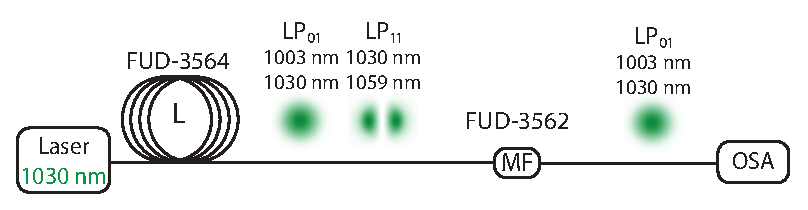
\includegraphics[width=0.8\linewidth]{Dissertation/images/imfwm/scheme_osa.eps}
	\caption{Экспериментальная установка для определения спектрального состава излучения в поперечной моде $\LPii$. MF: модовый фильтр; OSA: анализатор спектра.}
	\label{fig:synopsis_scheme_osa}
\end{figure}

\begin{figure}[th]
	\centering
	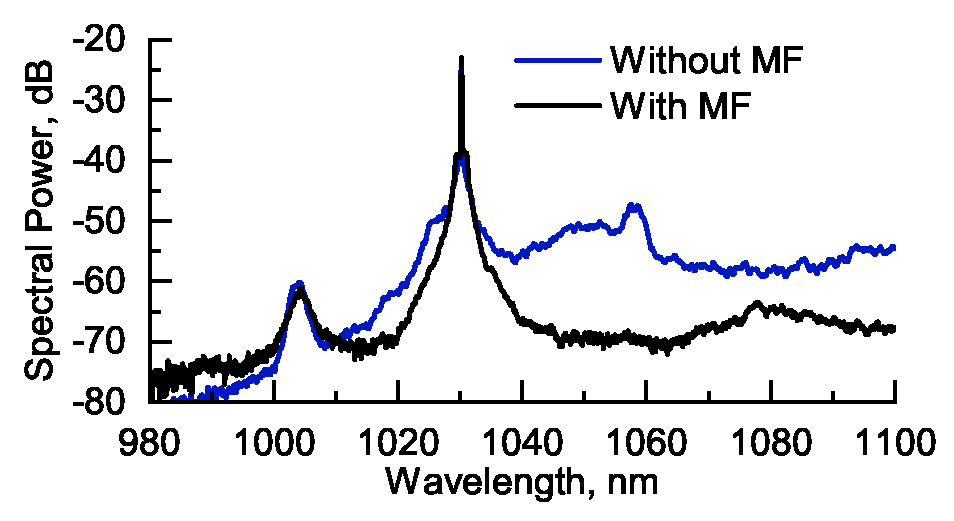
\includegraphics[width=0.6\linewidth]{Dissertation/images/imfwm/mode_filter_spectra}
	\caption{Спектры в области $1~\text{мкм}$ с применением (чёрный) и без применения (синий) МФ.}
	\label{fig:synopsis_mode_filter_spectra}
\end{figure}

На рисунке~\cref{fig:synopsis_mode_filter_spectra} синяя и чёрная кривые соответствуют выходным спектрам с применением и без применения МФ соответственно. В спектральных областях $1030~\text{нм}$ (накачка) и $1003~\text{нм}$ (антистоксовая компонента) различия между спектрами минимальны (менее $0.5~\text{дБ}$), что указывает на сохранение этих компонент при распространении излучения через МФ. В спектральной области около $1059~\text{нм}$ (стоксовая компонента) применение МФ привело к существенному ослаблению излучения на $20~\text{дБ}$. Это свидетельствует о присутствии моды $\LPii$ в данной спектральной области.


Второй метод основан на визуализации поперечного распределение интенсивности излучения в спектральной области 1059~нм. Схема эксперимента, визуализация пучка и его спектра показаны на рис.~\cref{fig:synopsis_scheme_mirror_lp11_spectra}.

\begin{figure}[th]
	\centering
	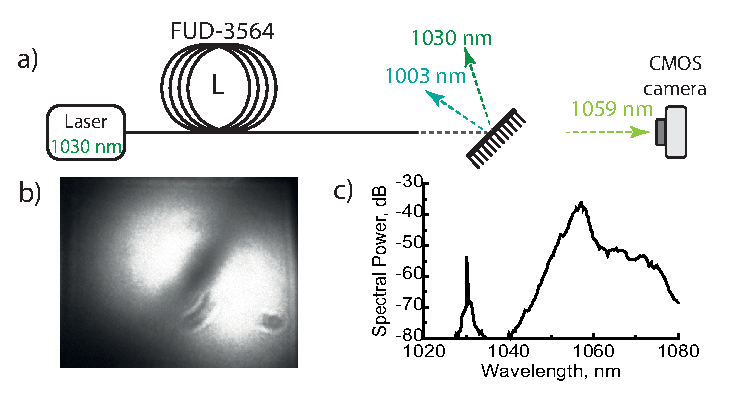
\includegraphics[width=0.8\linewidth]{Dissertation/images/imfwm/scheme_mirror.eps}
	\caption{a) Экспериментальная установка для визуализации пучка на длине волны $1059$~нм; b) изображение пучка на длине волны $1059$~нм; c) спектр после дихроичного зеркала.}
	\label{fig:synopsis_scheme_mirror_lp11_spectra}
\end{figure}

В экспериментальной установке использовалось дихроичное зеркало для разделения излучения в спектральных диапазонах 1000--1040~нм и 1050--1070~нм. Визуализация пучка на длине волны 1059~нм с помощью КМОП-камеры показала двухлепестковое распределение интенсивности, соответствующее поперечной моде $\LPii$.

Взаимное влияние ММЧВС в области 1 мкм и ОМЧВС между волнами накачки и затравки, показано в эксперименте, блок-схема которого показана на рис.~\cref{fig:synopsis_scheme_power}.

\begin{figure}[thbp]
	\centering
	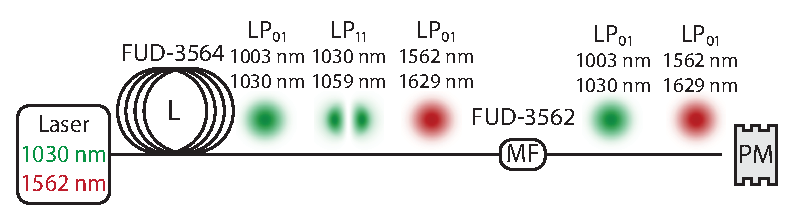
\includegraphics[width=0.8\linewidth]{Dissertation/images/imfwm/scheme_power.eps}
	\caption{Экспериментальная установка для измерения доли оптической мощности моды $\LPii$. MF: модовый фильтр; PM: измеритель мощности.}
	\label{fig:synopsis_scheme_power}
\end{figure}

\begin{figure}[thbp]
	\centering
	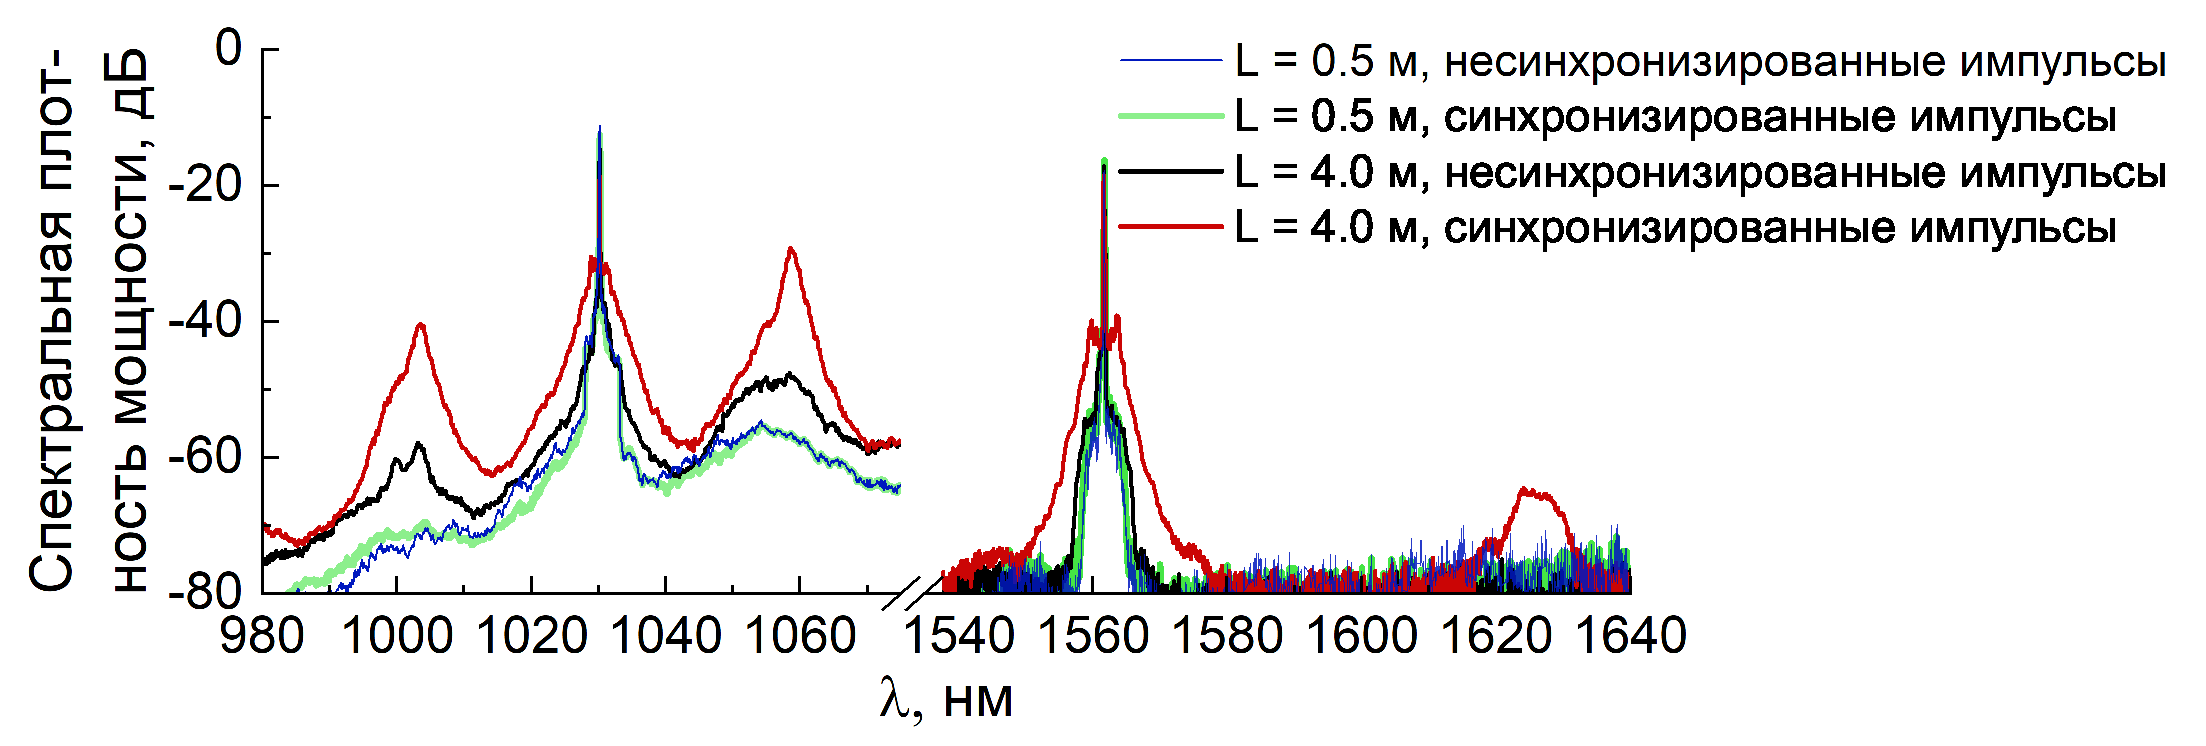
\includegraphics[width=0.95\linewidth]{Dissertation/images/imfwm/problem.eps}
	\caption{Измеренные спектры двухволнового лазера. $L$: длина ОВ}
	\label{fig:synopsis_problem}
\end{figure}

Спектры излучения синхронизированных и несинхронизированных импульсов накачки и сигнала показаны на рис.~\cref{fig:synopsis_problem}. Из них следует, что при одновременном распространении синхронизированных импульсов по ОВ доставки длиной 4~м на 20~дБ возрастает спектральная мощность не только антистоксовой компоненты ММЧВС на длине волны 1003~нм, но и стоксовой компоненты на длине волны 1059~нм. Также были измерены зависимости доли мощности моды $\LPii$ от длины волокна доставки для случаев синхронизированных и несинхронизированных импульсов накачки и затравки. Показано, что синхронизация импульсов приводит к увеличению доли высшей моды в диапазоне длин ОВ от 1~м 4~м.

Таким образом, экспериментально показано, что в исследуемом ОВ доставки достигается взаимное влияние двух процессов ЧВС, развивающихся по следующим схемам:

\begin{equation}
	\LPoi^{1030}+\LPii^{1030}\longrightarrow \LPoi^{1003}+\LPii^{1059}
	\label{eq:synopsis_schemeIMFWM}
\end{equation}
\begin{equation}
	\LPoi^{1030}+\LPoi^{1562}\longrightarrow \LPoi^{1003}+\LPoi^{1629}	
	\label{eq:synopsis_schemeFWM}
\end{equation}

В~\cref{eq:synopsis_schemeIMFWM,eq:synopsis_schemeFWM} нижний индекс соответствует номеру поперечной моды, верхний индекс соответствует длине волны в нм.

Экспериментальные результаты подтверждены теоретической моделью, описывающая взаимодействие ОМЧВС и ММЧВС в ОВ доставки. Модель основана на системе связанных нелинейных уравнений распространения для четырёх взаимодействующих волн с учётом интегралов перекрытия поперечных мод. Для ММЧВС, развивающегося по схеме~\cref{eq:synopsis_schemeIMFWM}, и ОМЧВС по схеме~\cref{eq:synopsis_schemeFWM}, рассчитаны кривые фазового синхронизма и спектры параметрического усиления. Показано, что оба процесса имеют общую антистоксову компоненту на длине волны 1003~нм в моде $\LPoi$, что приводит к перекрытию их спектров усиления и взаимному усилению.

\begin{figure}[h]
	\centering
	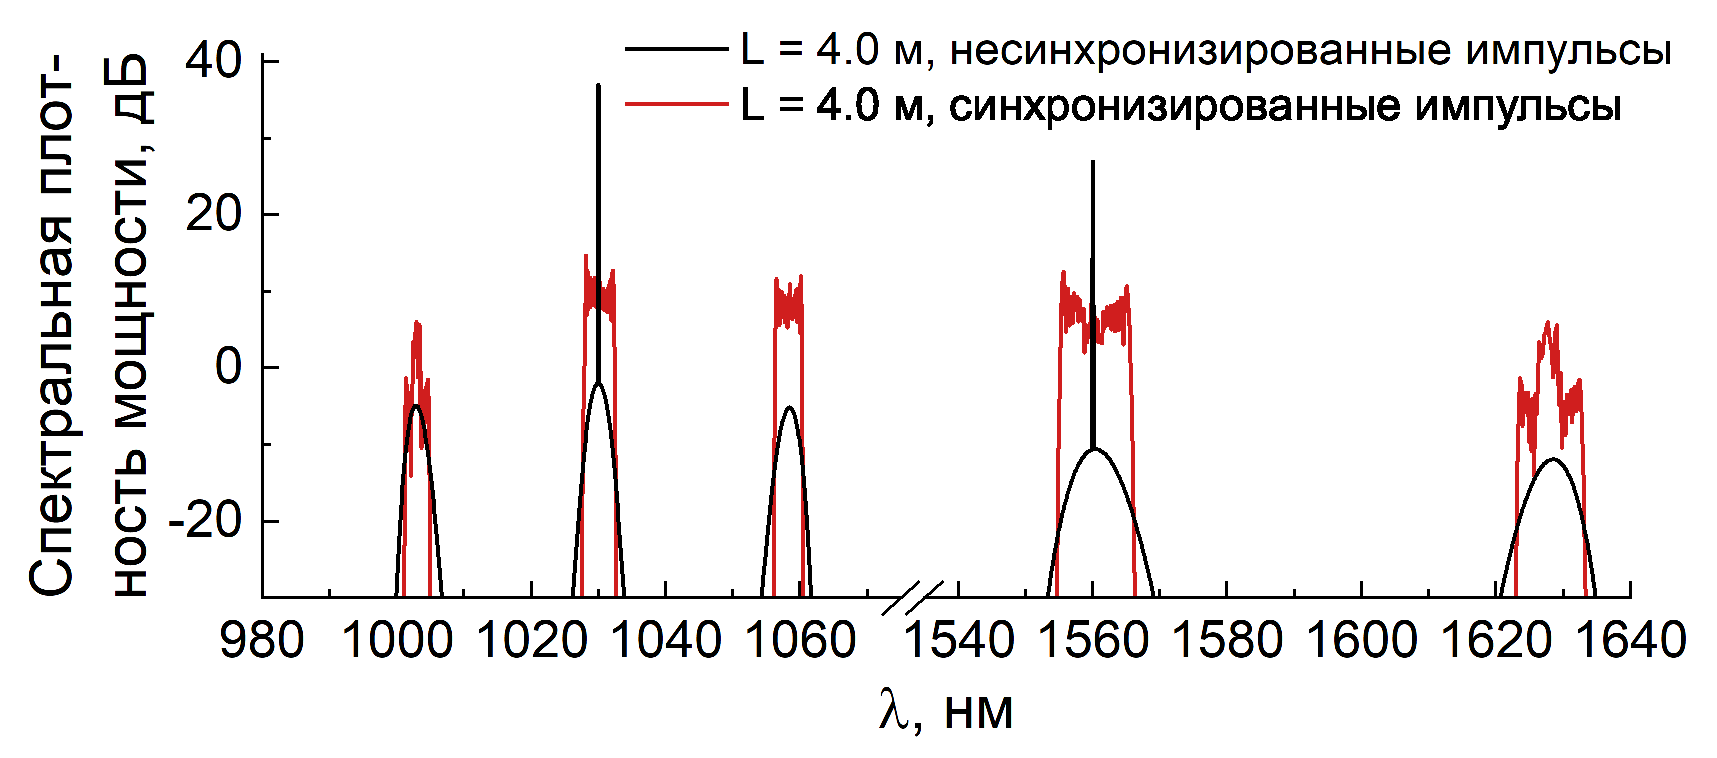
\includegraphics[width=0.85\linewidth]{Dissertation/images/imfwm/model_spectra.eps}
	\caption{Рассчитанные спектры двухволнового лазера для несинхронизированных (только ММЧВС, чёрный) и синхронизированных (ОМЧВС и ММЧВС, красный) импульсов}
	\label{fig:synopsis_model_spectra}
\end{figure}


ПРО ПОДАВЛЕНИЕ












\underline{\textbf{Вторая глава}} посвящена исследованию

\underline{\textbf{Третья глава}} посвящена исследованию

Можно сослаться на свои работы в автореферате. Для этого в файле
\verb!Synopsis/setup.tex! необходимо присвоить положительное значение
счётчику \verb!\setcounter{usefootcite}{1}!. В таком случае ссылки на
работы других авторов будут подстрочными.
Изложенные в третьей главе результаты опубликованы в~\cite{vakbib1, vakbib2}.
Использование подстрочных ссылок внутри таблиц может вызывать проблемы.

В \underline{\textbf{четвертой главе}} приведено описание

\FloatBarrier
\pdfbookmark{Заключение}{conclusion}                                  % Закладка pdf
В \underline{\textbf{заключении}} приведены основные результаты работы, которые заключаются в следующем:
%% Согласно ГОСТ Р 7.0.11-2011:
%% 5.3.3 В заключении диссертации излагают итоги выполненного исследования, рекомендации, перспективы дальнейшей разработки темы.
%% 9.2.3 В заключении автореферата диссертации излагают итоги данного исследования, рекомендации и перспективы дальнейшей разработки темы.
\begin{enumerate}
  \item При создании гибридного источника излучения на длине волны 3 мкм с волоконной накачкой в маломодовом ОВ доставки впервые обнаружено взаимное влияние ОМЧВС и ММЧВС, имеющих общую антистоксовую компоненту на длине волны 1003~нм. Показано, что синхронизация импульсов накачки (1030~нм) и затравки (1562~нм) увеличивает спектральную мощность компонент ММЧВС на 20 дБ, что впоследствии снижает эффективность ГРЧ в н-о кристалле. Предложен и реализован метод подавления взаимного влияния ЧВС с помощью модового фильтра на входе ОВ, позволяющий увеличить допустимую длину ОВ доставки с 2.5 м до 3.0 м без существенной потери полезной мощности накачки.
  \item Впервые экспериментально исследована эволюция КФС при фотоиндуцированной ГВГ в германосиликатном ОВ в режиме самозатравки. Показано, что в процессе оптического полинга ширина КФС и их сдвиг монотонно уменьшаются до стационарных значений, а форма кривых сохраняет выраженную асимметрию. Проведён соответствующий численный расчёт с использованием модели~\cite{antonyuk2001self} с добавлением учёта керровского эффекта. Обнаружено, что на поздних стадиях эффективность ГВГ остаётся практически постоянной вследствие динамического равновесия между уменьшением спектральной расстройки и ростом пиковой эффективности преобразования. Полученные результаты создают основу для разработки физической модели фотоиндуцированной ГВГ в ОВ, которая позволит прогнозировать уровень паразитной ГВГ в ОВ доставки мощных лазеров, в которых данный эффект может быть нежелательным, поскольку он может приводить к снижению порога оптического разрушения н-о кристаллов при ГРЧ в гибридных лазерных системах.
  \item Предложены поправочные выражения для трёх методик обработки температурных кинетик при разогреве образца лазерным излучением в методе ЛК, позволяющие компенсировать нестабильность температуры окружающей среды и коэффициента теплоотдачи. Экспериментально показано, что применение поправок снижает разброс измеренных значений коэффициента оптического поглощения более чем в два раза (с 23\% до 11\%).
\end{enumerate}


\pdfbookmark{Литература}{bibliography}                                % Закладка pdf
При использовании пакета \verb!biblatex! список публикаций автора по теме
диссертации формируется в разделе <<\publications>>\ файла
\verb!common/characteristic.tex!  при помощи команды \verb!\nocite!

\ifdefmacro{\microtypesetup}{\microtypesetup{protrusion=false}}{} % не рекомендуется применять пакет микротипографики к автоматически генерируемому списку литературы
\urlstyle{rm}                               % ссылки URL обычным шрифтом
\ifnumequal{\value{bibliosel}}{0}{% Встроенная реализация с загрузкой файла через движок bibtex8
    \renewcommand{\bibname}{\large \bibtitleauthor}
    \nocite{*}
    \insertbiblioauthor           % Подключаем Bib-базы
    %\insertbiblioexternal   % !!! bibtex не умеет работать с несколькими библиографиями !!!
}{% Реализация пакетом biblatex через движок biber
    % Цитирования.
    %  * Порядок перечисления определяет порядок в библиографии (только внутри подраздела, если `\insertbiblioauthorgrouped`).
    %  * Если не соблюдать порядок "как для \printbibliography", нумерация в `\insertbiblioauthor` будет кривой.
    %  * Если цитировать каждый источник отдельной командой --- найти некоторые ошибки будет проще.
    %
    %% authorvak
%    \nocite{vakbib1}%
%    \nocite{vakbib2}%
%    \nocite{vakbib3}%
%    \nocite{vakbib4}%
%    \nocite{vakbib5}%
%    \nocite{vakbib6}%
%    \nocite{vakbib7}%
%    \nocite{vakbib8}%
%    \nocite{vakbib9}%
%    \nocite{vakbib10}%
%    \nocite{vakbib11}%
%    \nocite{vakbib12}%
    %
    %% authorwos
    \nocite{zotov2025}
    \nocite{ostapiv2023mutual}
    \nocite{ostapiv2026evolution}
%    \nocite{wosbib1}%
    %
    %% authorscopus
%    \nocite{scbib1}%
    %
    %% authorpatent
%    \nocite{patbib1}%
    %
    %% authorprogram
%    \nocite{progbib1}%
    %
    %% authorconf
	\nocite{ostapiv2025phase}
	\nocite{ostapiv_kinetics}
	\nocite{iclo2022imfwm}
	\nocite{mephi2022imfwm}
	\nocite{mipt2022shgfiber}
	\nocite{llph2023imfwm}
	\nocite{samara2023imfwm}
	\nocite{mipt66gradient}
	\nocite{iclo2024gradient_theory}
	\nocite{iclo2024gradient_exp}
	\nocite{mipt67shg_fiber}
	\nocite{ostapiv2021determination}
    %
    %% authorother
%    \nocite{bib1}%
%    \nocite{bib2}%

    \ifnumgreater{\value{usefootcite}}{0}{
        \begin{refcontext}[labelprefix={}]
            \ifnum \value{bibgrouped}>0
                \insertbiblioauthorgrouped    % Вывод всех работ автора, сгруппированных по источникам
            \else
                \insertbiblioauthor      % Вывод всех работ автора
            \fi
        \end{refcontext}
    }{
        \ifnum \totvalue{citeexternal}>0
            \begin{refcontext}[labelprefix=A]
                \ifnum \value{bibgrouped}>0
                    \insertbiblioauthorgrouped    % Вывод всех работ автора, сгруппированных по источникам
                \else
                    \insertbiblioauthor      % Вывод всех работ автора
                \fi
            \end{refcontext}
        \else
            \ifnum \value{bibgrouped}>0
                \insertbiblioauthorgrouped    % Вывод всех работ автора, сгруппированных по источникам
            \else
                \insertbiblioauthor      % Вывод всех работ автора
            \fi
        \fi
        %  \insertbiblioauthorimportant  % Вывод наиболее значимых работ автора (определяется в файле characteristic во второй section)
        \begin{refcontext}[labelprefix={}]
            \insertbiblioexternal            % Вывод списка литературы, на которую ссылались в тексте автореферата
        \end{refcontext}
        % Невидимый библиографический список для подсчёта количества внешних публикаций
        % Используется, чтобы убрать приставку "А" у работ автора, если в автореферате нет
        % цитирований внешних источников.
        \printbibliography[heading=nobibheading, section=0, env=countexternal, keyword=biblioexternal, resetnumbers=true]%
    }
}
\ifdefmacro{\microtypesetup}{\microtypesetup{protrusion=true}}{}
\urlstyle{tt}                               % возвращаем установки шрифта ссылок URL
